\documentclass{article}
\usepackage[table]{xcolor}
\usepackage{float}
\usepackage{array}
\usepackage{graphicx}
\usepackage[spanish, es-tabla]{babel}
\usepackage[utf8]{inputenc}
\usepackage{csquotes}
\usepackage[margin=1.55cm]{geometry}
\usepackage{wallpaper}
\usepackage[depth=3]{bookmark}
\usepackage[
backend=biber,
style=numeric,
sorting=none
]{biblatex}
\bibliography{references}
%\addbibresource{references.bib} 
\setlength{\parskip}{1em}
\parindent 0px

\newcolumntype{P}[1]{>{\centering\arraybackslash}p{#1}}
\newcolumntype{M}[1]{>{\centering\arraybackslash}m{#1}}
 

\newcommand\signature{
\noindent\begin{minipage}{10cm}
    \noindent\vspace{3pt}\par
    Firma: \rule{7cm}{1pt}
    \noindent\vspace{15pt}\par
\end{minipage}}

\begin{document}

\begin{titlepage}


    \ThisLRCornerWallPaper{1}{imgs/fondo_tt.png} % Fondo de portada 
        \begin{center}
            \LARGE \textbf{Instituto Politécnico Nacional}\\*[0.3cm]
            \Large \textbf{Escuela Superior de Cómputo}\\
            \vspace{1cm}
            \rule{12cm}{0.5mm}\\*[0.3cm]% Línea {Longitud}{Grosor}
            \hspace{0.9cm} 
            %\normalsize {\textit{Ingeniería en Sistemas Computacionales}}\\
            %%%%  TITULO Y NÚMERO DE TRABAJO   %%%%
    		\LARGE \textbf{ Aplicación móvil gamificada de aritmética\\}
    		\LARGE \textbf {\emph{Trabajo Terminal No 2021-1-007}} 
    		\vspace{1cm} %Espacio vertical
    	\LARGE \textbf{\\ Ingeniería en Sistemas Computacionales\\}
    	Alumnos: *Pineda Vieyra Itzcoatl Rodrigo, Mothelet Delgado Izaird Alexander\\
	Directores: Elena Fabiola Ruiz Ledesma, Lorena Chavarría Baez\\
	e-mail: itzcoatlpv@gmail.com
    \vspace{1cm} %Espacio vertical
        \end{center}

    \centering %Todo centrado
    \vspace{1cm} %Espacio vertical

    %%%%   ALUMNOS   %%%%
   	


\end{titlepage}

\tableofcontents
\pagebreak
\section{Introducción}
La intervención educativa requiere de una previa comprensión de la adquisición y desarrollo de la competencia aritmética
que está en la base de todas las posteriores dificultades y trastornos del aprendizaje matemático. Hay dificultades que
pueden surgir a lo largo de este proceso(desde nivel básico), lo que repercute en la resolución de ejercicios y problemas matemáticos avanzados.
Por lo que el desarrollo de la destreza operatoria aritmética es fundamental para que el estudiante, tanto de nivel básico como medio superior, pueda enfrentar con
éxito situaciones más complejas en el campo de la Matemática. Además, se requiere motivar al estudiante al desarrollar
trabajo operatorio aritmético, ya que en ocasiones su desarrollo puede resultar monótono y aburrido. Para ayudar al desarrollo de la destreza operatoria de los estudiantes se propone una aplicación gamificada móvil que promueva la
resolución de ejercicios aritméticos.

\subsection{Motivación}
La Aritmética como la Geometría son de las disciplinas matemáticas más antiguas y necesarias en la historia del género humano \cite{coronado2014estudio}. 
Su utilización funcional es requerida para las personas que participamos de esta sociedad, como medio de comunicación y comprensión de multitud de fenómenos que nos rodean, es por ello que el desarrollo de la destreza operatoria aritmética es una de las habilidades más necesitadas en la alfabetización socio instrumental.
Los niveles de fracaso en el aprendizaje matemático son preocupantes, especialmente en los últimos cursos de escolaridad obligatoria (secundaria). Los resultados de estudios internacionales como el Programa Internacional para la Evaluación de Alumnos de la OCDE (PISA)\cite{oecd2014what,oecd2016low} muestran que el aprendizaje matemático es el que presenta mayor porcentaje de fracaso \cite{coronado2016academic, mullis2016timss}. El cálculo es un componente esencial en la resolución de problemas aritméticos, y éste es uno de los contenidos más importantes de las matemáticas, junto a la geometría, la medida o la probabilidad. 
Es por ello que un elevado porcentaje de las dificultades de aprendizaje de las matemáticas tiene un origen aritmético, donde el cálculo representa un papel esencial \cite{orrantia2006dificultades}. Las habilidades numéricas y aritméticas son predictores críticos del futuro éxito o fracaso académico matemático\cite{rodriguez2017marcadores}. 

Se ha observado en declive las habilidades operatorias aritméticas de estudiantes universitarios\cite{tariq2002decline,carpenter2017psychology,huang2013gamification}. 
El estudiante cree que podrá contar con la calculadora de su celular en todo momento, pero cuando esto no se le permite, como en los exámenes de admisión, la falta del entrenamiento del cálculo mental entorpece la solución correcta de los reactivos 
de dichos exámenes. Por otra parte, el no fortalecer la destreza operatoria, afecta diferentes procesos cognitivos al llegar a la edad adulta\cite{martin2003loss}.
El presentar al estudiante los ejercicios de una forma rutinaria muchas veces provoca aburrimiento y desmotivación. 
También es fundamental la motivación y el estado emocional de los estudiantes en su desempeño académico. La motivación y estado emocional de los estudiantes es un factor clave en su desempeño académico\cite{larrazolo2013habilidades,ryan1997should}. Si deseamos que los jóvenes 
mexicanos tengan un mejor desempeño en el área de las Matemáticas, se requiere presentarles 
distintas formas de aprender y practicar sus conocimientos. Para ello una estrategia de 
apoyo es la gamificación, la cual se empleará para incentivar a los estudiantes de educación 
media superior a desarrollar su destreza operatoria.

\subsection{Plantamiento del Problema}
La problemática que se pretende atacar es la necesidad de fortalecer la destreza operatoria aritmética de los estudiantes de nivel básico y  medio superior [13], [14], lo cual es importante para el desarrollo del pensamiento matemático de los estudiantes. 
\subsection{Objetivos}
\subsubsection{Objetivo General}Desarrollar una aplicación móvil que apoye al estudiante de nivel básico y  medio superior en la 
adquisición de habilidades y conocimientos elementales, para fortalecer la destreza 
operatoria en  Aritmética, con el uso de la gamificación.

\subsubsection{Objetivos Específicos}
\begin{itemize}
	\item Diseñar actividades gamificadas, empleando números enteros con las 4 operaciones básicas.
	\item Desarrollar un módulo evaluador expresiones.
	\item Desarrollar un módulo de logros y mecánicas.
	\item Validar la aplicación móvil. 
\end{itemize}
\subsection{Estado del Arte}
El trabajo realizado en torno a la gamificación en los últimos años es considerablemente extenso, siendo aplicado en diferentes ambientes, demográficas y propósitos. Para el presente documento nos enfocaremos en el trabajo relacionado a su aplicación en el ámbito matemático.

En Brazil se creó una platofortma interactiva en linea enfocada a ayudar a estudiantes de nivel medio en sus lecciones de matemáticas y como entrenamiento para la Olimpiada Brazileña de Escuelas Públicas (Olimpiada Brasileira de Matematica das Escolas Pablicas - OBMEP). El sistema permite a los alumnos resolver problemas generados aleatoriamente y divididos en tres temas principales, que son: Aritmética, Geometría y Combinatoria. El sistema pretende que el alumno resuelva un número determinado de problemas para entender los algoritmos y la lógica que hay detrás. También está vinculado con conceptos de gamificación para involucrar a los estudiantes en las actividades propuestas \cite{toda2014project}.

En un estudio canadiense propone una familia de rompecabezas que gamifican la práctica de la aritmética. Los rompecabezas se diseñan con un algoritmo evolutivo que constituye una instancia de generación automática de contenidos. Se definieron dos clases de rompecabezas: aquellos en los que la solución óptima utiliza todas las piezas y aquellos en los que la solución óptima no utiliza al menos una pieza.\cite{foxcroft2020polyomino}.

En el siguiente estudio se experimentó con tres tipos diferentes de actividades de aprendizaje gamificado(competitivo, colaborativo y adaptativo), en alummnos de segundo grado y de tercero que utilizaban tabletas y lecciones de aprendizaje digital para aprender matemáticas.Los niveles de rendimiento fueron significativamente más altos en una condición de gamificación que combinaba competición, narrativa y adaptabilidad con elementos de juego de rendimiento individual. Concluyen con el hecho de que la gamificación funcione o no no es el resultado de los elementos individuales del juego, sino la consecuencia de su combinación equilibrada. \cite{jaguvst2018examining}.
 
Un estudio argentino desarrolló una aplicación Android llamada Moravec con 150 niveles con 20 problemas cada uno, donde se requieren 15 respuestas correctas en determinado tiempo para avanzar al ssiguiente nivel. Concluyen que se puede motivar a los participantes a realizar un entrenamiento aritmético sustancial simplemente presentándolo en un formato gamificado \cite{zimmerman2016arithmetic}.

\begin{table}[H]
\centering
\begin{tabular}{|c|M{6cm}|M{5cm}|}
\hline
Software & Características & Precio en el mercado \\ \hline

Fraction Challange & 
\begin{itemize}
	\item PVP local
	\item rondas con tiempos
\end{itemize} & 
Gratuito con micro transacciones \\ \hline


1+2=3 & 
\begin{itemize}
	\item Sumas y restas de enteros
	\item Tablas de liderato 
\end{itemize}& 
Gratuito \\ \hline


Fracciones calculadora & 
\begin{itemize}
	\item Calculadora de fracciones
\end{itemize}& 
Gratuito \\ \hline


Math Games & 
\begin{itemize}
	\item Logros
	\item Tablas de liderato
	\item Estadísticas
	\item Tutoriales de como realizar operaciones básicas
\end{itemize} & 
Gratuito con contenido bloqueado(se puede desbloquear haciendo un pago único) \\ \hline

Arithmetic Practice & 
\begin{itemize}
	\item Logros
	\item Tablas de liderato
\end{itemize} & 
Gratuito con contenido bloqueado(se puede desbloquear haciendo un pago único) \\ \hline


Mental Arithmetic  & 
\begin{itemize}
	\item PVP local
	\item Logros
	\item Tablas de liderato
	\item Estadísticas
	\item Contenido desbloqueable
\end{itemize} & 
Gratuito \\ \hline

\end{tabular}
\label{tab:software}
\caption{Comparación con softwares disponibles.}
\end{table}
\subsection{Propuesta de Solución}
Con este proyecto se pretende ayudar al desarrollo de la destreza operatoria en la resolución de ejercicios aritméticos con números enteros haciendo uso de ciertos componentes de la gamificación (Logros) y mecánicas (Competición). Como futuros ingenieros en sistemas computacionales tenemos la responsabilidad de usar las habilidades para un benefficio social, por lo que deseamos unir esfuerzos para apoyar al estudiante a mejorar su destreza operatoria.
Los ejercicios podrán presentarse empleando preguntas de opción múltiple según la preferencia del usuario,
con la puntuación cambiando correspondientemente. Se contará con un sistema de puntuación basado en el tiempo de
respuesta para medir el desempeño. Esto con el propósito de fomentar la competitividad, permitiendo al estudiante llevar
un registro del progreso de su puntuación.
\section{Marco Teórico}
\subsection{Aritmética}
La aritmética es la parte de la matemática, referida a los números y a las operaciones y cálculos básicos que pueden realizarse con ellos: adición, sustracción, multiplicación y división. Su desarrollo es fruto de la madurez cognitiva del sujeto en la interacción con los objetos y la mediación de los instrumentos socioculturales de su contexto. El conocimiento de las operaciones básicas surge a partir de los aprendizajes informales y formales del conocimiento matemático.
Las investigaciones cognitivas que han estudiado el desarrollo de las habilidades para el cálculo, han establecido que esta competencia requiere de la integración de una serie de esquemas protocuantitativos [8], [9] con la experiencia de contar [10].
Esas estrategias de conteo que se utilizan inicialmente para sumar y restar, se van haciendo más complejas con el uso y la práctica, ampliándose a las operaciones de multiplicar y dividir, cuya práctica las hace interiorizarse en esquemas de memoria que posibilitarán posteriormente la recuperación de hechos numéricos (desde la memoria a largo plazo semántica) para la solución de operaciones de cálculo [10]-[12].


\subsection{Gamificación}
La Gamificación es comúnmente definida como “El uso de técnicas, elementos y dinámicas propias de los juegos en contextos que no son de juego, con el fin de potenciar la motivación, así como de reforzar la conducta para solucionar un problema, mejorar la productividad, obtener un objetivo, activar el aprendizaje” \cite{robson2015all}. Donde un juego está definido como “un sistema formal basado en reglas con un resultado variable y cuantificable, donde a los diferentes resultados se les asignan valores diferentes, el jugador se esfuerza para influir en el resultado, el jugador se siente apegado al resultado y las consecuencias de la actividad son opcionales y negociables” \cite{zichermann2011gamification}.
La gamificación emplea distintos tipos de recompensas para fomentar los comportamientos deseados. Estas recompensas pueden generalizarse con el acrónimo SAPS.
\begin{itemize}
	\item Status, reconocimiento. Las tablas de puntuación (leaderboards) son un ejemplo.
	\item Acceso,ofrecen la posibilidad de acceder a un punto o a algo a lo que los otros individuos no pueden.
	\item Poder, ejemplo en foros donde aquellos con más puntos no tienen que pasar por la revisión.
	\item Cosas (Stuff), recompensas tangibles. 
\end{itemize}

La gamificación ha sido explorada principalmente para su aplicación en empresas, definiendo dinámicas y estrategias que aumenten la productividad de los empleados. Sin embargo, la aplicación que nos compete es su potencial dentro de la educación. Como ya se mencionó anteriormente, la mayoría de estudios y aplicaciones han trabajado en los niveles más elementales de educación (primaria)\cite{rodrigues2017math}. Esto no quiere decir que no se haya intentado a niveles superiores o que hayan fracasado \cite{wiggins2016overview,sanchez2017classcraft,tan2018}, incluso se ha usado
en carreras afines a la de Ingeniería a Sistemas Computacionales \cite{ibanez2014gamification}. Sin importar el nivel académico, si
se cuenta con un buen diseño, la gamificación puede resultar una estrategia muy útil. Los elementos de
gamificación que se busca integrar a este Trabajo Terminal, son:
Tablas de liderato.
Sistema de puntuación.
Logros.
Dichos elementos son algunos de los más comunes y que han demostrado impactan la motivación de los
estudiantes en los estudios revisados \cite{wiggins2016overview,sanchez2017classcraft,ibanez2014gamification,tan2018}
\section{Análisis}
\subsection{Requisitos Funcionales}
\begin{enumerate}
\item {El sistema permitirá el registro de usuarios, este se realizará por medio de un correo electrónico y contraseña válidos.}
\item{El sistema permitirá el ingreso de un usuario al sistema mediante un correo y contraseña  previamente registrados.}
\item {El sistema permitirá el registro y acceso mediante una cuenta de Google.}
\item {El sistema contará con un modo de juego infinito, un modo por tiempo y un modo de jugador contraa jugador local}
\item{El sistema permitirá a los uuarios elegir que tipo de operaciones realizar asi como la dificultad}
\item{Los administradores podrán añadir plantillas con los respectivoss valores que se usarán}
\end{enumerate}
\subsection{Requisitos No Funcionales}
\begin{enumerate}
\item {La aplicación no deberá exceder 2 GB de almacenamiento}
\item {La aplicación deberá ser compatible con Android 8.1 en adelante}
\item {Los ejercicios deberán generarse en menos de 2 segundos}
\item {La aplicación podrá ser usada por cualquier usuario con al menos 10 minutos de instruccción}
\item {Se requerirá conexión a internet.}
\item {La aplicación contará con escabilidad para otros temas.}
\item {Las interfaaces deberán estar optimizadas para dispositivos móviles.}
\end{enumerate}
\subsection{Casos de Uso}
%diagrama de casos de uso
\begin{figure}[H]
    \centering
    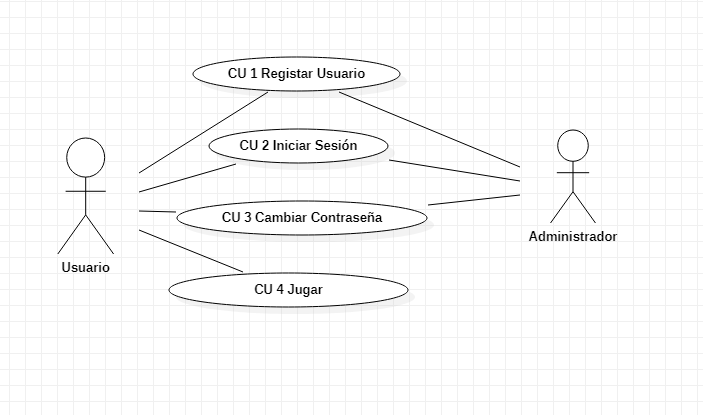
\includegraphics[scale=0.7]{imgs/CasosDeUso}
    \caption{Diagrama de Casos de Uso}
\end{figure}
\subsubsection{Tabla descriptiva de Caso de Uso 1}
\begin{tabular}{|M{5cm}|c|}
\hline
Caso de Uso & CU1 Registrar Usuario\\ \hline
Versión & 1.1\\ \hline
Autor(es) & Itzcoatl Rodrigo Pineda Vieyra\\ \hline
Revisor & Izaird Alexander Mothelet Delgado \\ \hline
Actor(es) & Usuario Final \\ \hline
Entradas & correo electrónico, contraseña, \\ & Cuenta de Google \\ \hline
Salidas & Cuenta de usuario creada \\ \hline
Pre-condiciones & Instalar y abrir la aplicación \\ \hline
Post-condiciones & Cuenta de usuario creada\\ \hline
Mensajes & MSN1: "Ingrese un texto válido"\\
		 & MSN2: "Bienvenido"\\ \hline
Fuente & RF1,RF3 \\ \hline	
	Trayectoria & Trayectoria A (principal)\\
		& 1.   El usuario seleccionará la opción de registrarse.\\
		& 2.   Se ingresarán los datos correspondientes.\\
		& 3.   Se creará correctamente la cuenta del usuario\\
		& 4.   Se envia un correo de confirmación al email proporcionado \\	
	& Trayectoria B\\
	& 1.   El usuario seleccionará la opción de registrarse.\\
	& 2.   Se proporcionará una cuenta de Google\\
	& 3.   Se confirma y se dan los permisos correspondientes.\\
	& 4   Se creará correctamente la cuenta del usuario.\\ \hline
\end{tabular}
\subsubsection{Tabla descriptiva de Caso de Uso 2}
\begin{tabular}{|M{5cm}|c|}
\hline
Caso de Uso & CU2 Iniciar Sesión\\ \hline
Versión & 1.1\\ \hline
Autor(es) & Itzcoatl Rodrigo Pineda Vieyra\\ \hline
Revisor & Izaird Alexander Mothelet Delgado \\ \hline
Actor(es) & Usuario Final \\ & Administrador\\ \hline
Entradas &  Correo electrónico, contraseña\\ & Cuenta de Google \\ \hline
Salidas & Sesión de usuario \\ \hline
Pre-condiciones & Instalar y abrir la aplicación \\ \hline
Post-condiciones & Sesión iniciada\\ \hline
Mensajes & MSN1: "Ingrese un texto válido"\\
		   & MSN2: "Bienvenido"\\ \hline
Fuente & RF2,RF3 \\ \hline	
	Trayectoria & Trayectoria A (principal)\\
		& 1.   El usuario ingresa sus credenciales (correo y contraseña).\\
		& 2.   Se valida si existen coincidencias de las credenciales proporcionadas\\
		& 3. Se inicia sesión o se despliega un mensaje de error.\\
	& Trayectoria B\\
	& 1.   El usuario seleccionará la opción de registrarse.\\
	& 2.   Se proporcionará una cuenta de Google\\
	& 3.   Se inicia sesión.\\ \hline
\end{tabular}
\subsubsection{Tabla descriptiva de Caso de Uso 3}
\begin{tabular}{|M{5cm}|c|}
\hline
Caso de Uso & CU3 Cambiar Contraseña\\ \hline
Versión & 1.1\\ \hline
Autor(es) & Itzcoatl Rodrigo Pineda Vieyra\\ \hline
Revisor & Izaird Alexander Mothelet Delgado \\ \hline
Actor(es) & Usuario Final \\ \hline
Entradas &  Correo y contraseña nueva \\ \hline
Salidas & Cuenta con ccontraeña nueva \\ \hline
Pre-condiciones & Iniciar Sesión \\ \hline
Post-condiciones & \\ \hline
Mensajes & MSN1: "Se envio el correo para reestablecer contraseña"\\
		   & MSN2: "Bienvenido"\\ \hline
Fuente & RF4 \\ \hline	
	Trayectoria
		& 1.	El usuario selecciona el Modo Infinito del menu lateral\\
		& 2.    El usuario responde  las preguntas \\
		& 3.	El usuario comete 3 errores o presiona el boton de regreso, terminando el juego.\\ \hline
\end{tabular}
\subsubsection{Tabla descriptiva de Caso de Uso 4}
\begin{tabular}{|M{5cm}|c|}
\hline
Caso de Uso & CU4 Jugar\\ \hline
Versión & 1.1\\ \hline
Autor(es) & Itzcoatl Rodrigo Pineda Vieyra\\ \hline
Revisor & Izaird Alexander Mothelet Delgado \\ \hline
Actor(es) & Usuario Final \\ \hline
Entradas &  Respuesta, modo de juego, operación, dificultad \\ \hline
Salidas & Puntuación \\ \hline
Pre-condiciones & Iniciar Sesión \\ \hline
Post-condiciones & Puntuación\\ \hline
Mensajes & \\
Fuente & RF4, RF5 \\ \hline	
	Trayectoria
		& 1.	El usuario selecciona Juegos del menu lateral o de la pantalla principal\\
		& 2. El usuario selecciona el modo de juego, el tipo de operaciones y la dificultad.\\
		& 3.    El usuario responde  las preguntas \\
		& 4.	Al completar la ronda de preguntas o cometer 3 errores en caaso del modo infinito, termina el juego.\\ 
		& 5. 	Se informa al usuario de su puntuación y se registra en el leaberboard\\ \hline
\end{tabular}
\subsubsection{Tabla descriptiva de Caso de Uso 5}
\begin{tabular}{|M{5cm}|c|}
\hline
Caso de Uso & CU5 Consultar Leaderboard\\ \hline
Versión & 1.1\\ \hline
Autor(es) & Itzcoatl Rodrigo Pineda Vieyra\\ \hline
Revisor & Izaird Alexander Mothelet Delgado \\ \hline
Actor(es) & Usuario Final \\ \hline
Entradas &  Modo de juego, operacion \\ \hline
Salidas & Leaderboard \\ \hline
Pre-condiciones & Iniciar Sesión\\ \hline
Post-condiciones & \\ \hline
Mensajes & \\
Fuente &  \\ \hline	
	Trayectoria
		& 1.	El usuario selecciona Leaderboards del menu lateral o de la pantalla principal \\
		& 2. El usuario selecciona el modo de juego, el tipo de operaciones.\\
		& 3.    El usuario responde  las preguntas \\
		& 4.	Se despliega el leaderboard correspondiente\\ \hline
\end{tabular}
\subsubsection{Tabla descriptiva de Caso de Uso 6}
\begin{tabular}{|M{5cm}|c|}
\hline
Caso de Uso & CU6 Consultar Logros\\ \hline
Versión & 1.1\\ \hline
Autor(es) & Itzcoatl Rodrigo Pineda Vieyra\\ \hline
Revisor & Izaird Alexander Mothelet Delgado \\ \hline
Actor(es) & Usuario Final \\ \hline
Entradas &  Modo de juego, operacion \\ \hline
Salidas & Leaderboard \\ \hline
Pre-condiciones & Iniciar Sesión,  \\ \hline
Post-condiciones & \\ \hline
Mensajes & \\
Fuente &  \\ \hline	
	Trayectoria
		& 1. El usuario selecciona Logros del menu lateral o de la pantalla principal \\
		& 2. Se despliega la lista de logros \\ \hline
\end{tabular}
\subsubsection{Tabla descriptiva de Caso de Uso 7}
\begin{tabular}{|M{5cm}|c|}
\hline
Caso de Uso & CU7 Subir Plantilla\\ \hline
Versión & 1.1\\ \hline
Autor(es) & Izaird Alexander Mothelet Delgado\\ \hline
Revisor &  Itzcoatl Rodrigo Pineda Vieyra \\ \hline
Actor(es) & Administrador \\ \hline
Entradas &  Plantilla, valores \\ \hline
Salidas & Leaderboard \\ \hline
Pre-condiciones & Iniciar Sesión \\ \hline
Post-condiciones & Plantilla en Base de Datos\\ \hline
Mensajes & \\
Fuente &  \\ \hline	
	Trayectoria
		& 1. El administrador selecciona Plantillas del menu lateral o de la pantalla principal \\
		& 2. Se despliega la lista de plantillas\\ 
		& 3. Se presiona el botón de + para agregar plantilla\\
		& 4. Se rellenan los campos de plantilla y valores respecctivos a  cada dificultad \\		
		\hline
		
\end{tabular}
\subsubsection{Tabla descriptiva de Caso de Uso 8}
\begin{tabular}{|M{5cm}|c|}
\hline
Caso de Uso & CU7 Otorgar permisos\\ \hline
Versión & 1.1\\ \hline
Autor(es) & Itzcoatl Rodrigo Pineda Vieyra \\ \hline
Revisor &  Izaird Alexander Mothelet Delgado \\ \hline
Actor(es) & Administrador \\ \hline
Entradas &  Plantilla, valores \\ \hline
Salidas & 1 \\ \hline
Pre-condiciones & Iniciar Sesión  \\ \hline
Post-condiciones & Usuario con permisos de adminitrador\\ \hline
Mensajes & \\
Fuente &  \\ \hline	
	Trayectoria
		& 1. El administrador selecciona Usuarios del menu lateral o de la pantalla principal \\
		& 2. Se despliega la lista de usuarios\\ 
		& 3. Se selecciona el usuario al que se desea otorgar o revocar permisos \\
		& 4. Se checa la checkbox para otorgar permisos\\
		& 5. Se selecciona la paloma para confirmar\\		
		\hline
\end{tabular}
\subsection{Análisis de Interfaces}
%Descripcion de tipo de interfaz y por que
Las interfaces deberán ser optimizadas para dispositivos móviles. Deberá considerarse la capacidad touch de dichos dispositivos. La primera pantalla será para Iniciar sesión por medio del correo y contraseña junto con un botón para registrarse. La pantalla de registro solicitará el correo, contraseña y confirmación de la contraseña. Se deberá contar con botones para acceder al perfil de usuario, leaderboards y logros en una barra de navegación, esta puede ser horizontal o vertical. La pantalla de ejercicios mostrará la puntuación en todo momento en una esquina y el número de respuestas correctas consecutivas junto un icono. En caso de haber tiempo para responder a una pregunta habrá una barra horizontal en la parte superior la cual irá desapareciendo conforme transcura el tiempo asignado al usuario para dar respuesta a la pregunta, la cual irá  desaapareciendo de derecha a izquierda.

\subsection{Análisis de la Base de Datos}%Narrativa
Para desarrollar esta aplicación se cuenta con una entidad Usuario con campos correo (llave primaria) y contraseña, con el correo como identificador de la entidad, pues no se permiten correos duplicados. Los Logros y leaderboards son manejaados por el servicio externo de Google Play Juegos por lo cual no se incluyen en nuestra base de datos.

\subsection{Análisis de Logros}
Los logros son una manera de inncentivar al jugador a cumplir ciertas metas, se decidió enfocarnos en pocos logros pero con un nivel de dificultad medio a difícil por recomedaación del siguiente estudio \cite{groening2019achievement}.
Los logros se desbloquearán automáticamente al llegar a cierta puntuación, racha, o  responder rápido. Al completar todos los logros el progreso no se reestableccerá. 


\subsection{Tecnologías usadas}
\subsubsection{Dart}
Dart es un lenguaje optimizado para el cliente que permite desarrollar 
aplicaciones rápidas en cualquier plataforma. Su objetivo es ofrecer el 
lenguaje de programación más productivo para el desarrollo multiplataforma, 
junto con una plataforma de ejecución flexible para marcos de aplicaciones.

Uno de los principales beneficios de usar Dart es su compilación AOT 
(Ahead-of-Time). AOT permite la capacidad de compilar código en código de 
máquina nativo. Como resultado, esto permite a los archivos binarios la 
capacidad de ejecutarse de forma nativa.

Además de ser muy flexible, fácil de usar y altamente compatible con Javascript, 
Dart permite que un programa se ejecute incluso si hay errores en otros lugares 
de la compilación. Esto permite a los desarrolladores la facilidad de edición 
ya que pueden probar sólo una pequeña sección del código sin importar si el 
resto de la aplicación está completa o no. 

Dart es un lenguaje rápido. Casi siempre compila más rápido, utilizando 
un compilador fuente a fuente. Puede esperar que tenga una interfaz de 
usuario más eficiente que muchos de los otros lenguajes principales.


\subsubsection{Flutter}
Flutter es un kit de herramientas de interfaz de usuario portátil para crear 
aplicaciones de tipo nativo en móviles, web y escritorio, a partir de una 
única base de código. Utiliza el lenguaje de programación Dart e incorpora 
Material Design y los widgets de Cupertino. Los desarrolladores de Flutter 
pueden crear una interfaz de usuario espectacular que se ve y se siente 
nativa. Se comporta de forma natural en cualquier plataforma, a pesar de 
que está utilizando una sola base de código.

Flutter es el único framework con un SDK para móviles que proporciona un 
estilo responsive sin utilizar un puente Javascript, alcanzando así un 
nivel de rendimiento que rivaliza con su primo y competidor directo 
React Native. Se integra fácilmente con las diferentes plataformas como 
Android, IOS y Linux, MAC, Windows y aplicaciones de Google Fuchsia.


\subsubsection{Firestore}
Firebase es un Backend-as-a-Service (Baas). Proporciona a los desarrolladores 
una variedad de herramientas y servicios para ayudarles a desarrollar aplicaciones 
de calidad. Está construido sobre la infraestructura de Google.

Firebase está categorizado como un programa de base de datos NoSQL, que almacena 
datos en documentos tipo JSON.

Firebase auth tiene un sistema de autenticación de correo electrónico/contraseña 
incorporado. También soporta OAuth2 para Google, Facebook, Twitter y GitHub. 
Nos centraremos en la autenticación de correo electrónico/contraseña en su mayor 
parte. 


%\subsubsection{Google Play Servicies}

\pagebreak
\section{Diseño}
\subsection{Arquitectura general del sistema}%Imagen arquitectura y descripcion%Imagen arquitectura y descripcion
La arquitectura se compone de 4 subsistemas (ver figura 2).  El primer subsistema es el de Registro e inicio de sesión y es el encargado de dar de alta y permitir el acceso a los usuarios ya registrados. El segundo subsistema corresponde a los módulos que interactuan con el usuario, estos son el módulo de ejercicios, encargado de proporcionar ejercicios al usuario, y el módulo evaluador de logros y mecánicas, el cual se encarga de llevar el registro de la puntuación, logros y niveles. El Subsistema de administardor incluye los módulos generador de problemas y evaluador de expresiones, los cuales se usan para generar los ejercicios para el usuario. También se incluye un módulo de actualización y consulta de dichos ejercicios. El último subsistema es el de estadísticas y progreso, el cual lleva el registro de los logros globales del usuario.  
\begin{figure}[H]
    \centering
    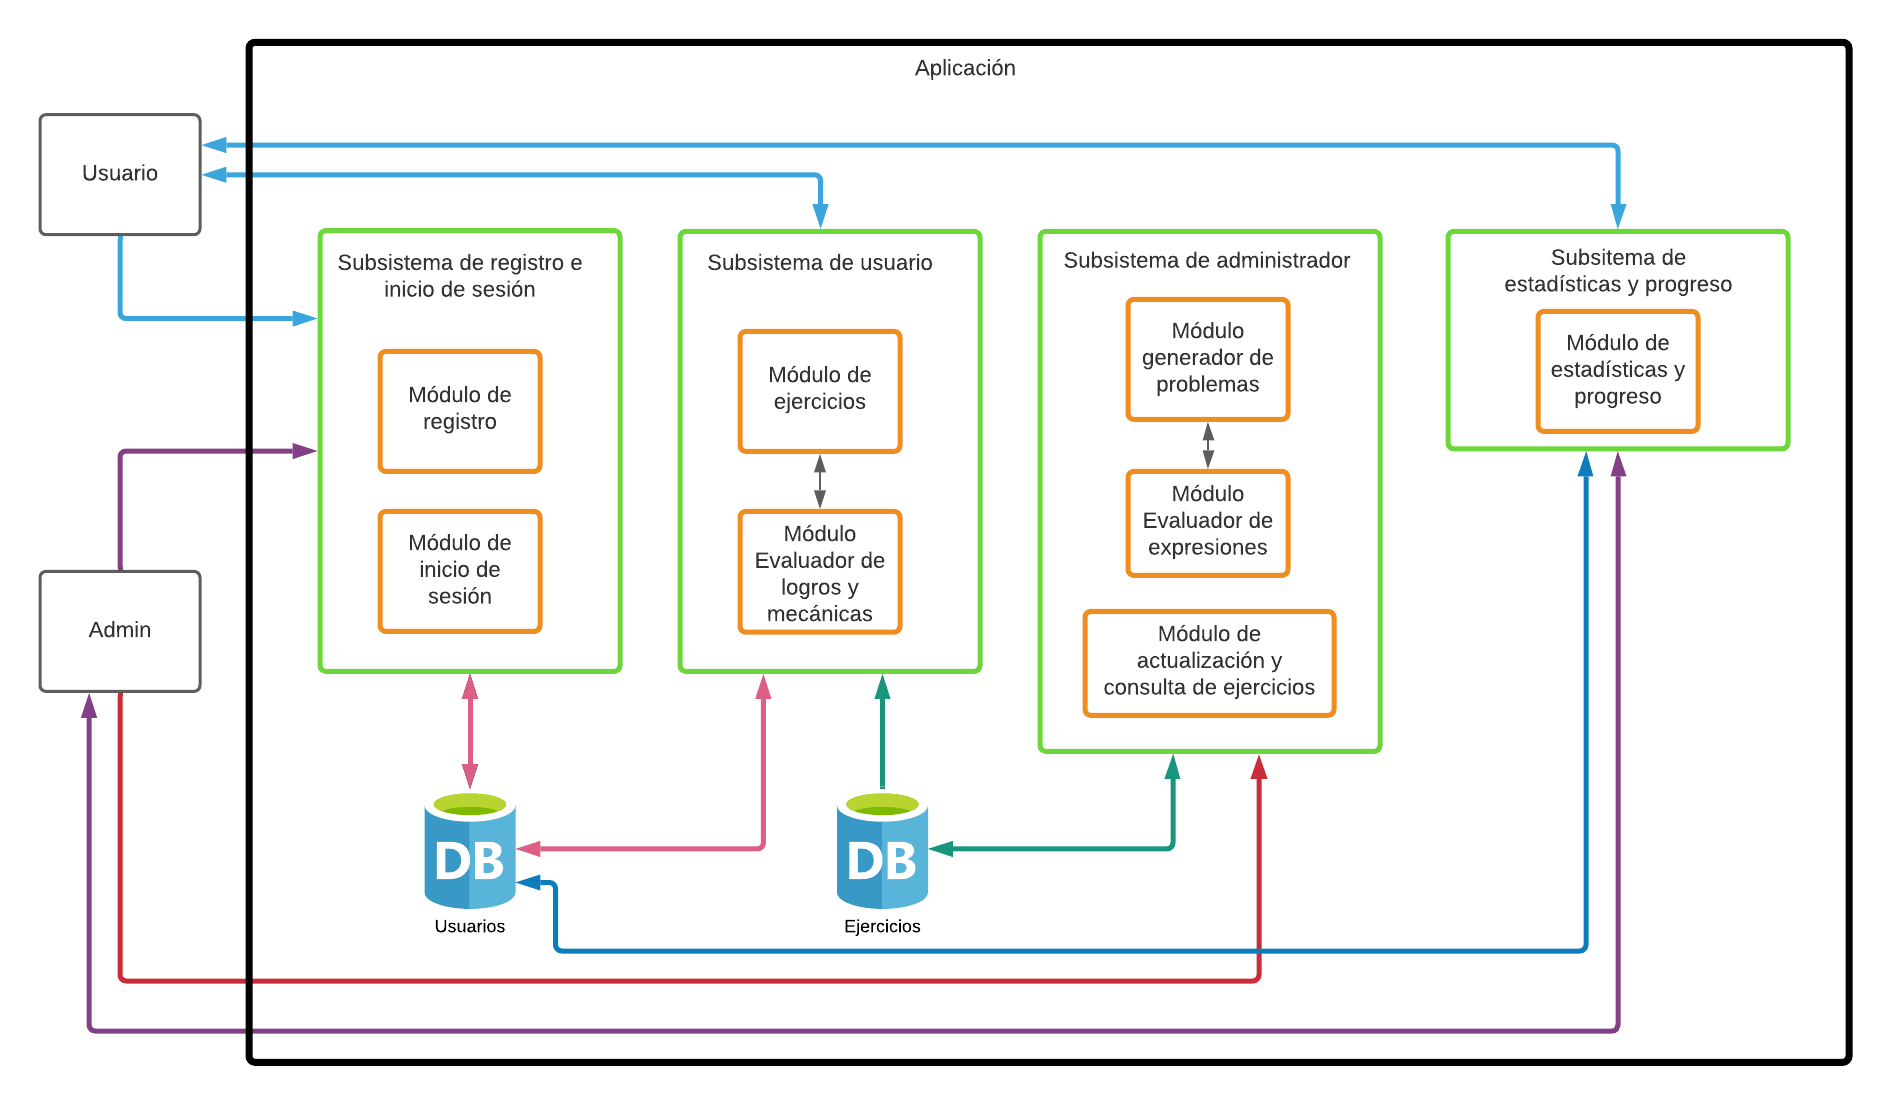
\includegraphics[scale=0.65]{imgs/Arquitectura}
    \caption{Arquitectura}
\end{figure}

\subsection{Diseño de Base de Datos}%diagrama entidad relacion pk subrayada
\begin{figure}[H]
    \centering
    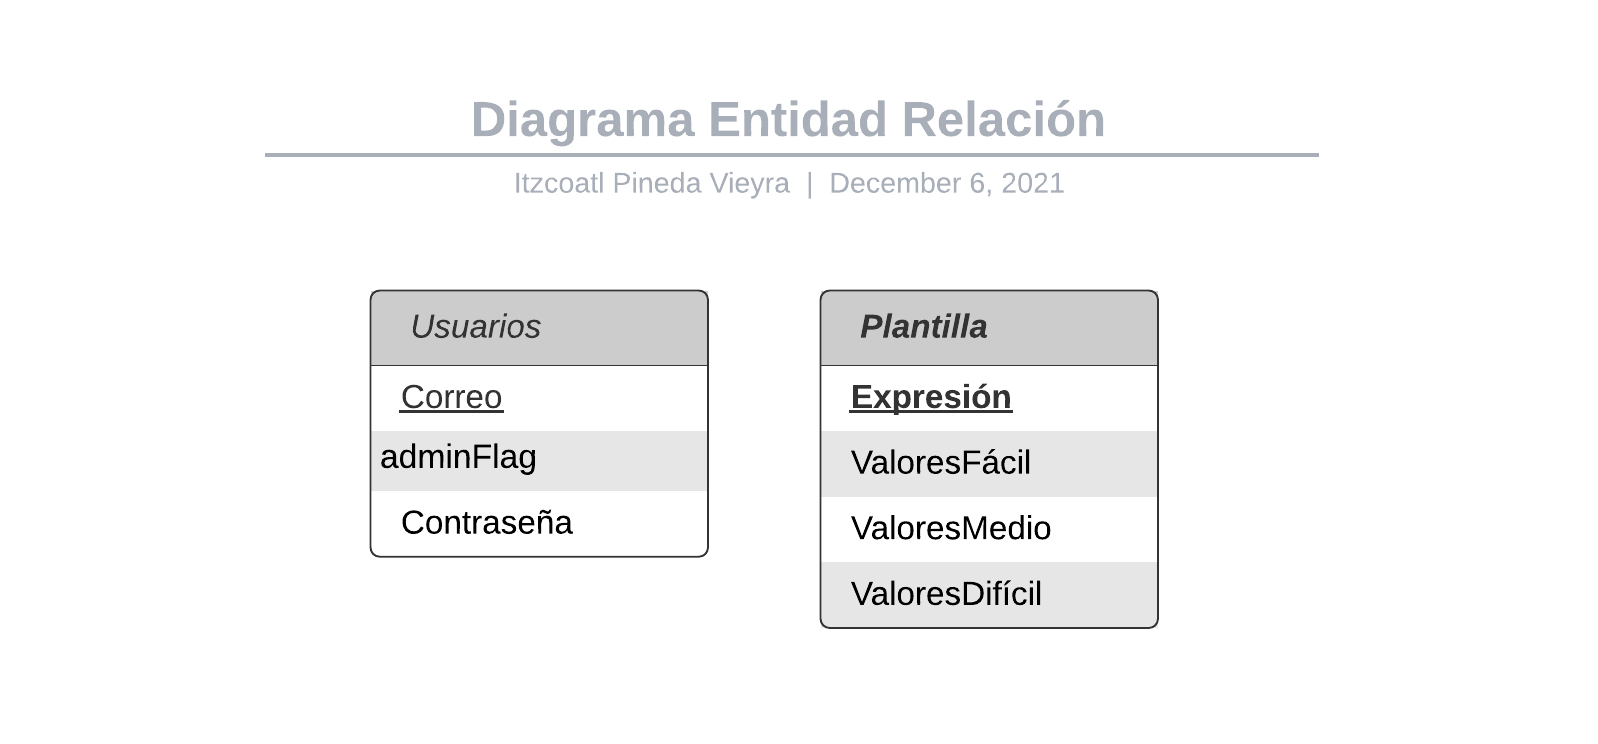
\includegraphics[scale=0.9]{imgs/BSD}
    \caption{Diagrama entidad relación}
\end{figure}
\subsection{Diseño de Base de Logros}
Los logros que se incluyeron fueron los siguienntes.

\begin{table}[H]

\begin{tabular}{|M{5cm}|c|}
\hline
Logro & Descripción\\ \hline
Inspirado & Consigue una racha de al menos 5 en el modo Infinito\\ \hline
Asendido & Consigue una racha de al menos 10 respuestas correctas en el modo Infinito\\ \hline
Perfeccioninsta & Responde correctamente todas las preguntas en una ronda del modo Clásico\\ \hline
Ágil &  Responde correctamente todas las preguntas en una ronda del modo Clásico\\ \hline
Veloz & En el modo Clásico, termina una partida en menos de 2 minutos con al menos 7 respuestas correctas.\\ \hline
Sub60s &   En el modo Clásico, termina una partida en menos de 1 minuto con al menos 7 respuestas correctas.\\ \hline
Académico & Consigue una puntuación de al menos 2,500 en el modo Clásico, dificultad Fácil\\ \hline
Estudioso & Consigue una puntuación de al menos 5,000 en el modo Clásico, dificultad Medio\\ \hline
Erudito & Consigue una puntuación de al menos 10,000 en el modo Clásico, dificultad Difícil\\ \hline
	
\end{tabular}
\label{tab:Logros}
\caption{Tabla de Logros}	
\end{table}
\subsection{Diseño de Interfaces}%mock-ups
En este apartado se presentarán los diseños de las interfaces previamente descritras.
\pagebreak
\begin{figure}[H]
    \centering
    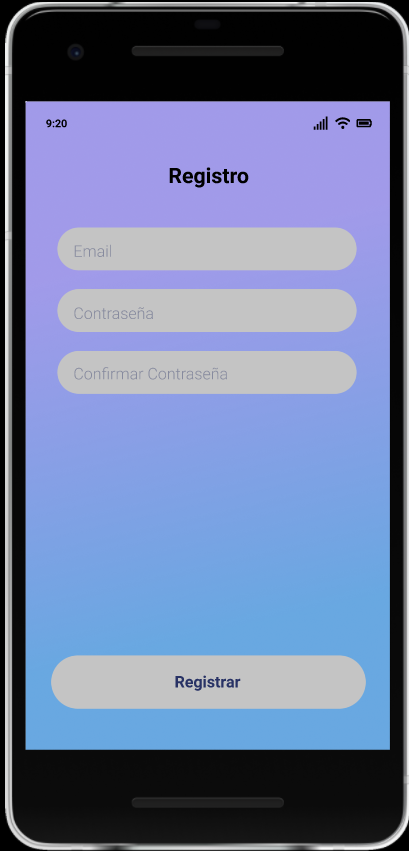
\includegraphics[scale=0.9]{imgs/Figma/Registro2} 
    \caption{Registro}
\end{figure}
\begin{figure}[H]
    \centering
    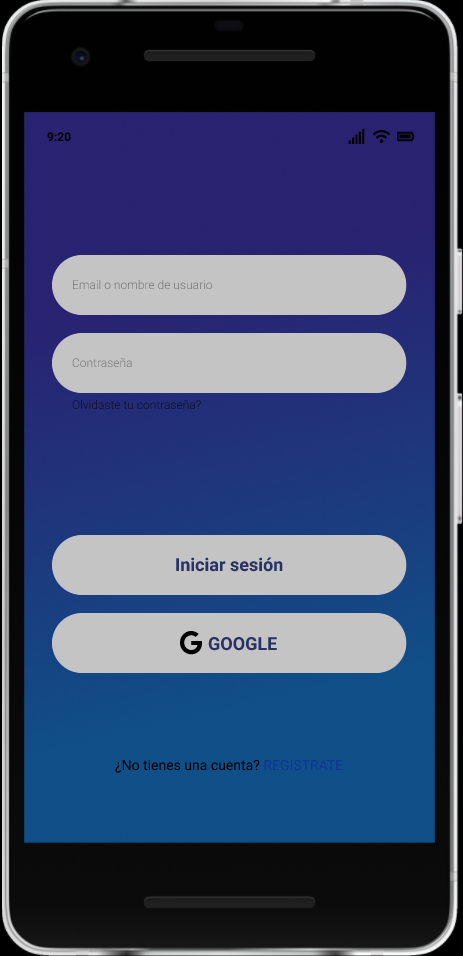
\includegraphics[scale=0.9]{imgs/Figma/Login}
    \caption{Login}
\end{figure}
\begin{figure}[H]
    \centering
    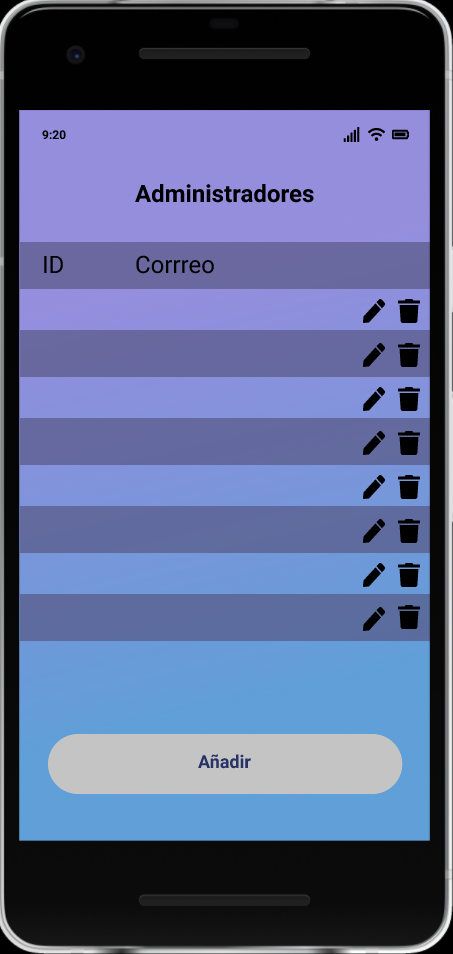
\includegraphics[scale=0.9]{imgs/Figma/Admins}
    \caption{Administrador}
\end{figure}
\begin{figure}[H]
    \centering
    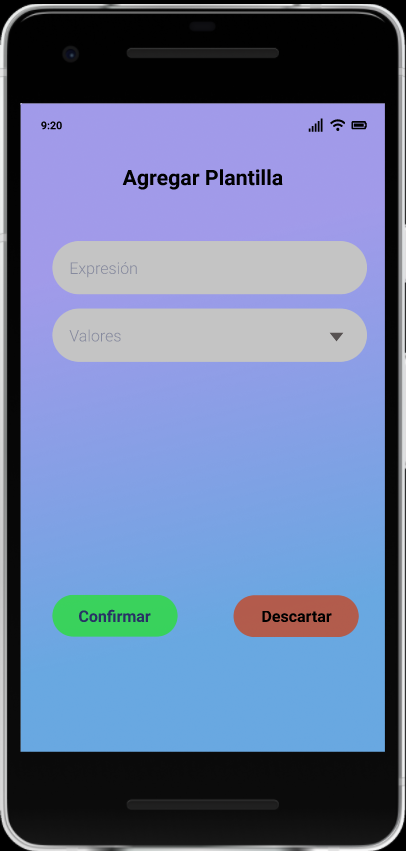
\includegraphics[scale=0.9]{imgs/Figma/Plantilla}
    \caption{Plantillas}
\end{figure}
\begin{figure}[H]
    \centering
    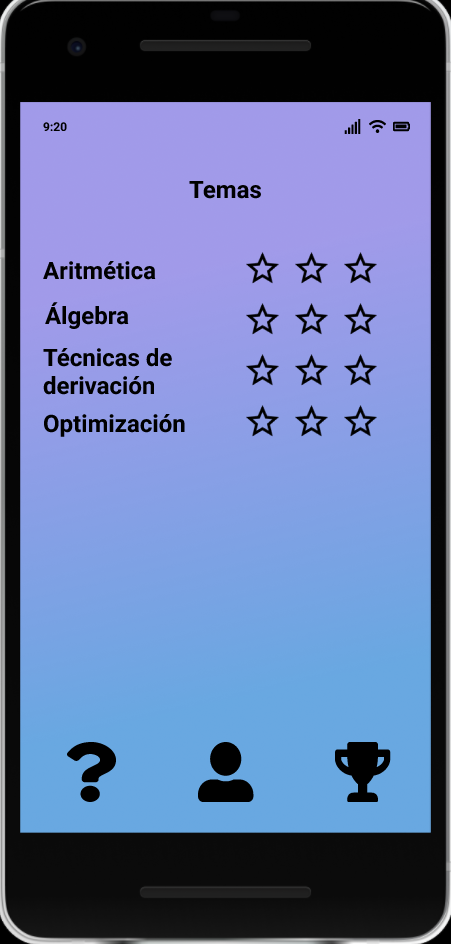
\includegraphics[scale=0.9]{imgs/Figma/Temas}
    \caption{Selección de tema}
\end{figure}
\begin{figure}[H]
    \centering
    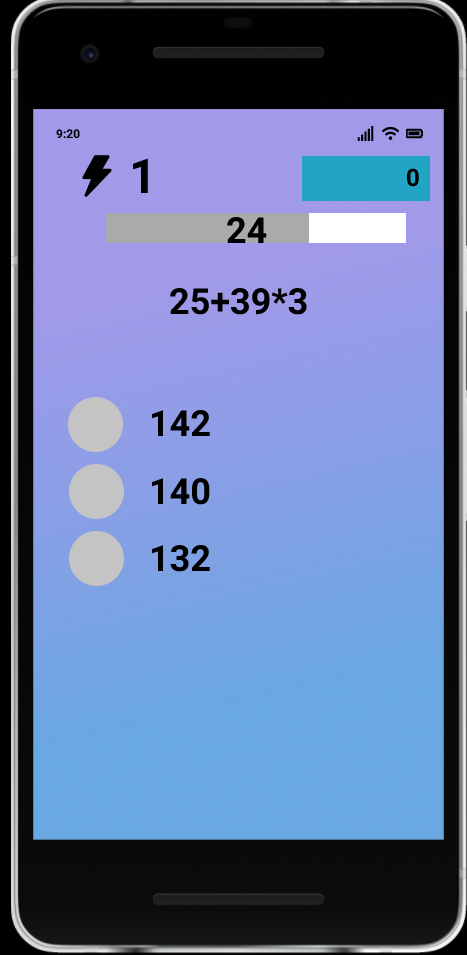
\includegraphics[scale=0.9]{imgs/Figma/Ejemplo}
    \caption{Ejemplo}
\end{figure}
\begin{figure}[H]
    \centering
    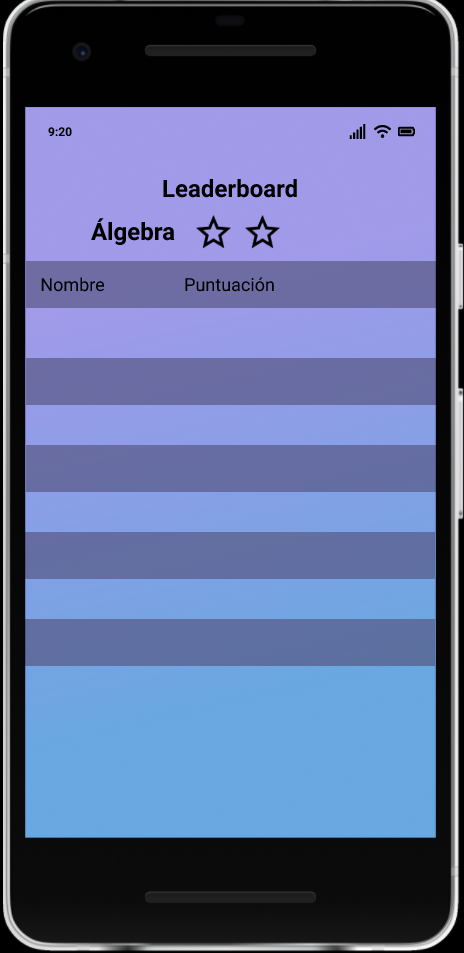
\includegraphics[scale=0.9]{imgs/Figma/Leaderboard}
    \caption{Leaderboard}
\end{figure}
\begin{figure}[H]
    \centering
    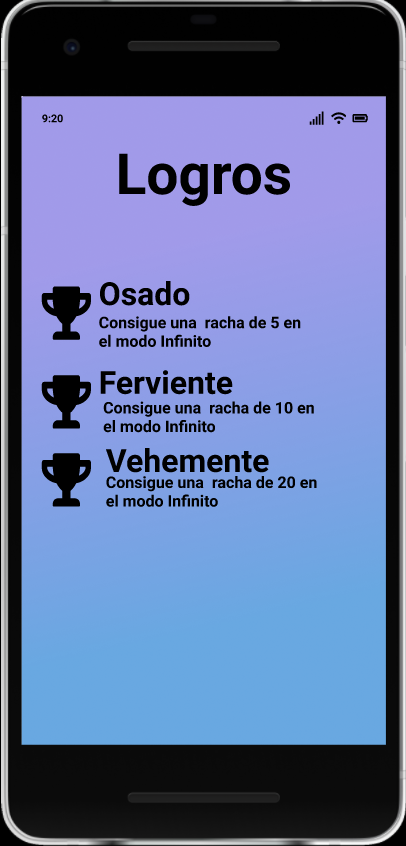
\includegraphics[scale=0.9]{imgs/Figma/Logros}
    \caption{Logros}
\end{figure}
\subsection{Metodología}
La metodología que se ha elegido para el desarrollo de este proyecto es Feature planninig 
\cite{hunt2006feature}, también conocida como Feature Driven 
Development F.D.D Esta metodología iterativa orientada a objetos, consistente en planear 
la estructura general del proyecto, realizar una lista de características, planear y finalmente 
construir cada una de ellas. En nuestro caso podemos ver cada característica como un tema y ciertas 
funcionalidades adicionales que deseamos integrar. Para garantizar la variedad de ejercicios se 
pretende usar técnicas de generación por procedimientos.

La lista de características sería la siguiente:
\begin{enumerate}
	\item Sistema de puntuación.
	\item Ejercicios de Aritmética.
	\begin{enumerate}
		\item Adición 
		\item Sustracción.
		\item Multiplicación.
		\item División.
	\end{enumerate}
	\item Evaluador de expresiones.
	\item Niveles de dificultades.
	\item Leaderboards.
	\item Estadísticas del jugador.
\end{enumerate}
\pagebreak
\section{Implementación}
%Subsistema de registro e ingreso Captura de pantalla con descripcion citar mock up de la pantalla
El subsistema de registro e ingreso fue implementado con Firebase 
\begin{figure}[H]
    \centering
    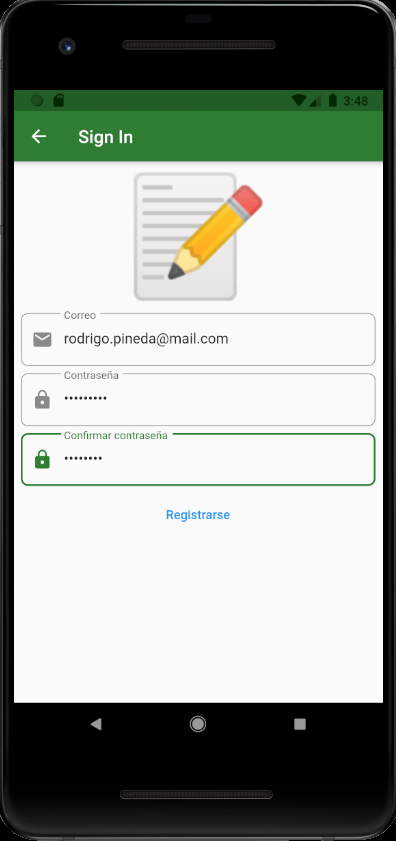
\includegraphics[scale=0.8]{imgs/Imp/Registro}
    \caption{Implementación Registro}
\end{figure}
\begin{figure}[H]
    \centering
    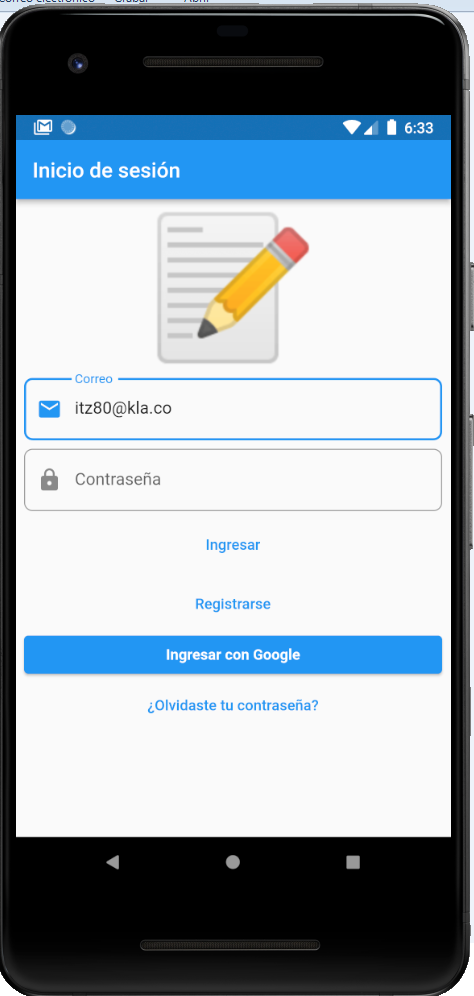
\includegraphics[scale=0.8]{imgs/Imp/Login1}
    \caption{Implementación de Login}
\end{figure}
\begin{figure}[H]
    \centering
    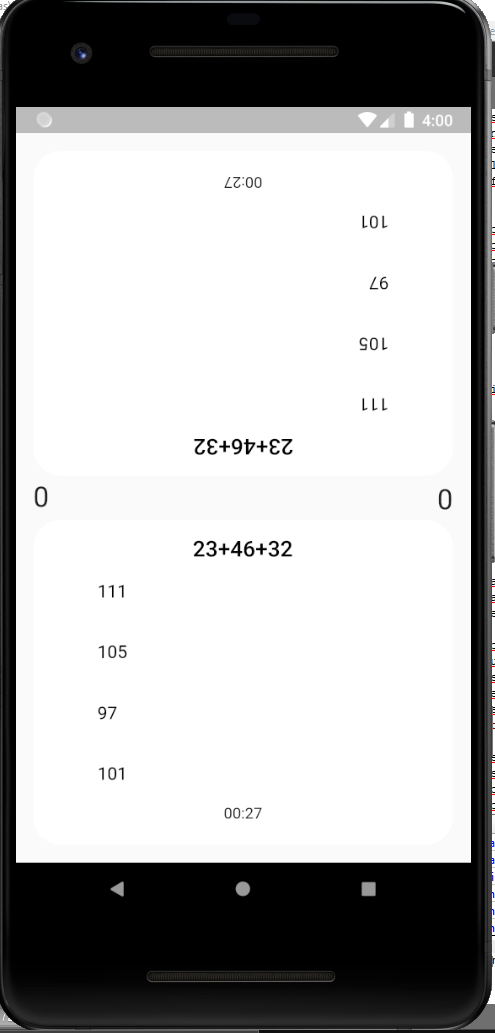
\includegraphics[scale=0.8]{imgs/Imp/Pvp}
    \caption{Implementación de modo jugador contra jugador}
\end{figure}
\begin{figure}[H]
    \centering
    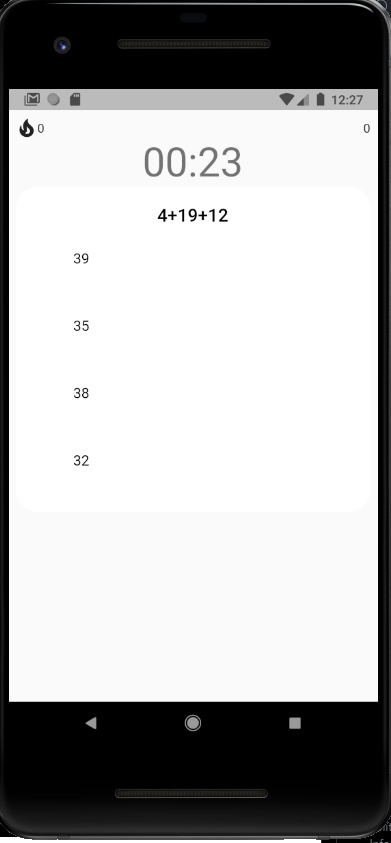
\includegraphics[scale=0.8]{imgs/Imp/Endless}
    \caption{Implementación de modo infinito}
\end{figure}
\begin{figure}[H]
    \centering
    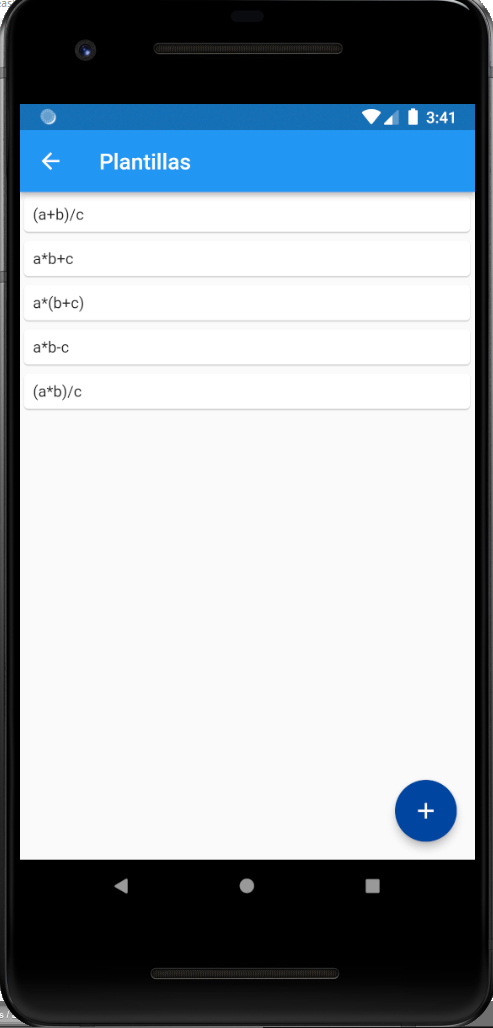
\includegraphics[scale=0.8]{imgs/Imp/Plantillas}
    \caption{Implementación de Plantillas}
\end{figure}
\begin{figure}[H]
    \centering
    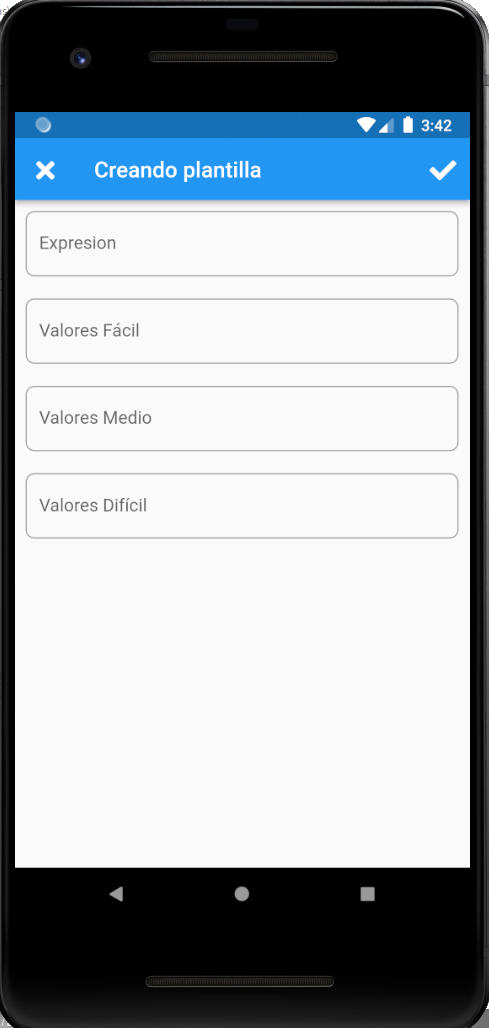
\includegraphics[scale=0.8]{imgs/Imp/Plantillas2}
    \caption{Implementación de Plantillas}
\end{figure}
\begin{figure}[H]
    \centering
    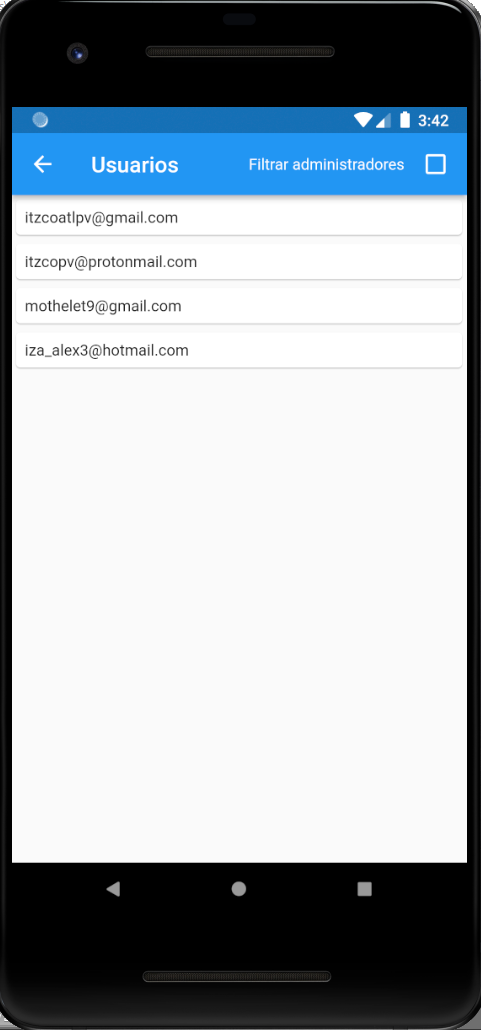
\includegraphics[scale=0.8]{imgs/Imp/Usuarios}
    \caption{Implementación de Usuarios}
\end{figure}
\begin{figure}[H]
    \centering
    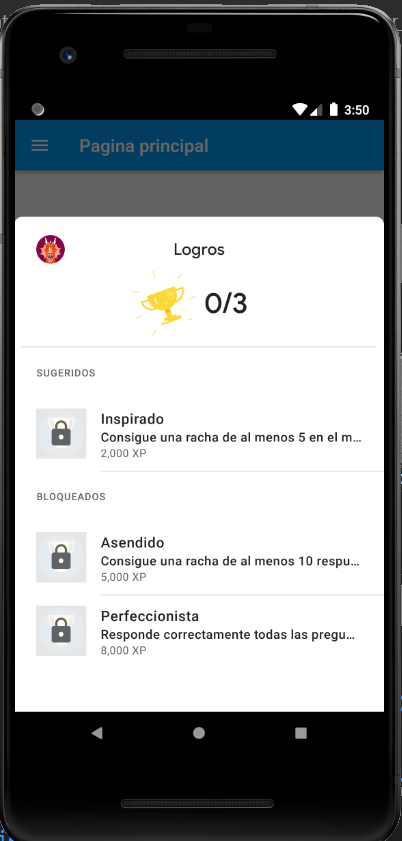
\includegraphics[scale=0.8]{imgs/Imp/Logros}
    \caption{Implementación de Logros}
\end{figure}
\begin{figure}[H]
    \centering
    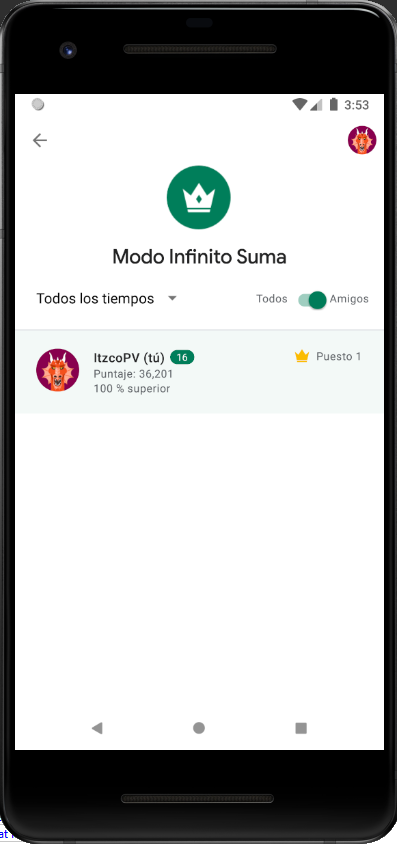
\includegraphics[scale=0.8]{imgs/Imp/Leaderboards}
    \caption{Implementación de Leadorboards}
\end{figure}
\section{Pruebas}%Que pruebas se le hicieron al sistema
Se validó el correo con una expresión regular. Algunos ejemplos de correos validos
\begin{itemize}
	\item itz80@kla.co
	\item \verb |itz!&*%^7@protonmail.net|
	\item 1A!e@protonmail.com
\end{itemize}

\pagebreak
\printbibliography


\end{document}